\section{Validation}\label{sec:validation}
The extent to which the minimization technique serves its diagnostic purpose is defined by its soundness, efficiency and, more importantly, information. 
The two main questions are:
\begin{description}
	\item[RQ1] Can it be applied efficiently in conjunction with other tools?	
	\item[RQ2] Does it help the engineer understand the cause of unrealizabity of their specification?
	\item[RQ3] How does the minimization structurally relates to the original automaton?		
\end{description}


%The presented diagnosis should help by pointing out the causes of non realizability, expressed in a language where the behavior of the plant, or as in this case a part of it, is explicit (). The diagnosis tool set should be a part of the specification process and must be present while progressively gathering knowledge and refining the model towards its intended form.

The measure of information our technique provides must be related to the impact it can have on the overall specification process, in particular in how clear it is for the engineer  to interpret the diagnosis. The aim is to minimize the amount of data presented while keeping it relevant to the unrealizability cause. The unavailability of skilled professionals and the amount of time and effort required to prepare a considerable set of external subjects up to the point where they would be able to write non trivial formal specifications, renders the perspective of a controlled experiment with external engineers writing specifications from scratch unfeasible. On the other hand, it is also impossible to propose a direct comparison with similar techniques, since, for instance, in ~\cite{DBLP:conf/hvc/KonighoferHB10} the minimization is applied on the set of environmental safety formulas, which in fact increments the volume of the plant when presented as an automaton, and in ~\cite{DBLP:conf/sigsoft/KuventMR17} a simplification of the symbolic counter strategy is presented as a LTS composed of attractors and trap states. We think that our technique adds a complimentary view to the non realizability diagnosis problem.

Research question \textbf{RQ1} is answered by the relation between synthesis and diagnosis time of similar specifications while \textbf{RQ2} is addressed by comparing the reduction volume of our technique with respect to the closest approach (~\cite{DBLP:conf/hvc/KonighoferHB10}). For \textbf{RQ3} we will study the correlation of the minimization amount against some structural properties of the original automaton.

We now explain the metrics used to quantitatively evaluate our technique. 
The first metric we compute is diagnosis time relative to the controller synthesis time ($t_{\mathcal{C}}=t_{E'}/t_{C}|$). The second metric is relative minimization volume ($v_{\mathcal{U}}$), defined as the size of the minimized plant against the original instance ($|\Delta_{E'}|/|\Delta_{E}|$). 
The number of transitions is used as the representation of absolute volume for two reasons, first, because it is a measure of how many options the user has when exploring the minimized plant, and the  second, because it is a dominant parameter in the complexity of the synthesis algorithms. 
The other metric we compute is minimization volume relative to the controller volume ($v_{\mathcal{C}}=|\Delta_{E'}|/|\Delta_{C}|$). The controller $C$ is the automaton representation of the strategy for the realizable version of each specification. The rationale behind this is that the size of the controller is a good proxy for the volume of the engineer's design intent in terms of concrete behavior. The motivation for taking the controller as a proxy of volume is that sometimes an ongoing specification is under defined, with weaker conditions than it will eventually have when reaching realizability. We expect our minimization to be at least comparable to the controller in terms of volume. We also measure relative controllability of the automaton as the sum of controllable options at each states over the total number of transitions.

In order to avoid bias, we used specifications taken from existing benchmarks and literature, prioritizing those where an unrealizable version was already present and mutating those were none was available in order to achieve unrelizability. 

%refs 
For each instance of those test cases we first wrote and synthesized the realizable version, and then modified it
to violate at least one of the original guarantees. 
These modifications are of two kinds, the first removes a required liveness assumptions from the original specification, the second relaxes a part of the environment by removing a safety environmental constraint. We assume that these modifications capture the way in which a model naturally evolves, the liveness omission stands for those situations where the environment is being mined for assumptions, which is both a partial and progressive process. The safety modification stands for those scenarios where the engineer is trying to figure out the explicit behavior of the plant, either by logically restricting the formula that describes it, or by defining and removing explicit transitions in a process-oriented syntax. In both cases unrealizability is introduced by constraining the system or relaxing the environment beyond its intended capabilities. We restrict ourselves to removing liveness assumptions under the premise that it is usually the case that the user has a clear intent of what the system should achieve (liveness guarantees) but needs to gain knowledge of the environment in which it will operate.  Because of this we are not considering the cases where unrealizability is caused by the fact that the guarantees are too strong. One variation per case is presented, in the parameterized examples, most of the liveness modifications produce symmetrical diagnosis. Our approach follows Cimatti's ~\cite{DBLP:conf/vmcai/CimattiRST08} in creating minimaly unfulfillable conflict by removing the smaller set of liveness assumptions to achieve non realizability.
 
Our benchmark is divided in two groups.The first group comes from the reactive synthesis domain, where behavior is described as a conjunction of safety formulae. These specifications usually describe hardware model and their symbolic nature allows for a concise and efficient representation and transformation of the model.  Our tool allows for such a specification to be properly written and it uses an intermediate ROBDD representation that is then translated into an explicit automaton before the synthesis/diagnosis steps are applied. The second goup comes from automata-based or process-based specifications, where a automaton representation of its behavior is almost straight-forward.

We will now briefly explain each case, show how they were parameterized and modified in order to achieve non realizability. 
The Generalized Buffer (GenBuf) and AMBA AHB case studies were taken from~\cite{DBLP:conf/hvc/KonighoferHB10}, the Lift Controller comes from ~\cite{DBLP:conf/fmcad/AlurMT13}, Collector is part of the SYNTCOMP competition ~\cite{SYNTCOMP} benchmark, Air Tower Control, Bidding Workflow, Cat and Mouse, Dining Philosophers, Travel Agency and Transfer Line are taken from ~\cite{ciolek2019compositional} where the authors collected several problems from the supervisory control domain, the exploration robot case was adapted from ~\cite{DBLP:journals/corr/abs-2001-07678}.
\begin{description}[align=left,leftmargin=0.7cm,font=\normalfont,style=nextline,itemsep=0pt]
\item[LC] The \textbf{Lift Controller} case specifies the behavior of a system that should eventually serve every request to take the elevator to a required floor when the corresponding button was pressed, and also to take it back to the ground floor if no request is pending. The parameter on these instances indicates how many floors are present in the specification. The \texttt{missing liveness} modification changes one of the liveness guarantees from $\square \Diamond (b_i \rightarrow f_i)$ to $\square \Diamond (f_i)$. The original form asks the system to serve a floor only when requested, the modification makes it serve a floor even when it was not requested. Due to other safety restrictions this renders the specification unrealizable. The \texttt{removed safety} modification allows an input signal to keep the elevator at a particular floor indefinitely.
\item[CO] The \textbf{Collector} case outputs a barrier signal once all inputs $in_1\ldots in_n$ have occurred at least once. The parameter indicates how many inputs the specification could receive. The \texttt{missing liveness} modification removes one of the assumptions that forces the environment to always eventually produce input $i$ ($\square\Diamond(in_i)$). The \texttt{removed safety} modification removes the relation between an input and an internal memory signal that is needed in order to keep track of the inputs read after the last barrier raise.
\item[GB] The \textbf{Generalized Buffer (GenBuf)} case has a FIFO for storing data incoming from senders, and a
controller to communicate with the senders, receivers, and the
FIFO. On the sender side, GenBuf receives a request input from each sender, and replies
with an acknowledge output. On the receiver side, GenBuf outputs a request and inputs an
acknowledge for each receiver. The GenBuf controller gets the \texttt{FULL} and \texttt{EMPTY} signals from the FIFO and
provides the \texttt{ENQ,DEQ}, and \texttt{SLC} signals for writing (reading) appropriate data to (from) the FIFO.
The parameter on each instance indicates how many senders the specification has. The \texttt{missing liveness} modification removes the assumption that the first receiver will eventually acknowledge a request, and in \texttt{removed safety} we removed original assumption \texttt{A5}, relaxing the behavior of the \texttt{FULL} and \texttt{EMPTY} signals.
\item[AB] The \textbf{AMBA AHB} defines a standard for on-chip communication between several devices operating in master-slave fashion. We split the arbiter in two modules, the \texttt{scheduler}, that is in charge of granting access to the masters and handling communication with the slaves, and the \texttt{burst manager}, that is in charge of handling signal burst operation. In this section we show the results for the \texttt{scheduler} since it is the only parameterized module of the two. 
The \texttt{missing liveness} modification removes the assumption that the \texttt{DECIDE} signal will always eventually be raised, which in turn does not assures that the scheduler will pick the next master to be served, and in \texttt{removed safety} the occurrence of \texttt{sel$_0$} fixes \texttt{hReq$_1$} to a low value, preventing the second master to be acknowledged. 
\item[ER] The \textbf{Exploration Robot} case models the behavior of a robot that can move through a sqare grid of size $n$, which also serves as the parameter for this specification. The robot must load cargo at the initial position and then unload it at the opposite corner of the grid. At the loading site the operation can either be successful or fail. The \texttt{missing liveness} modification removes the assumption that a load will always eventually occur. The \texttt{removed safety} modification allows the environment to neglect the load event indefinitely once a certain point in the grid is reached.
\item[TL] \textbf{Transfer Line} consists of $n$ machines
sequentially connected by $n$ buffers with finite capacity $k$, and an ending ma-
chine which may accept or reject a
finished product. The goal of the system is to process
elements avoiding buffer overflows and underflows. The
system controls when to input an element from buffer
$B_{i -1}$ into machine $M_i$ assuming infinite supply from
the outside world for $M_0$.
\item[DP] \textbf{Dinning Philosophers} is the classic concurrency
problem where $n$ philosophers are sitting around a table sharing
one fork with the adjacent philosopher. The goal of
the system is to control the access to the forks allowing
each philosopher to alternate between eating and thinking.
After grabbing a fork a philosopher needs to take $k$ intermediate
etiquette steps before eating. 
\item[CM] The \textbf{Cat and Mouse} case has $n$ cats
and $n$ mice placed in opposite ends of a corridor
divided in $2k +1$ cells. They take turns to move to one
adjacent area at a time, with mice moving first. The goal
of the system is to control the movement of mice in order
to avoid sharing an area with a cat (the movements of cats
are uncontrollable). In the center of the corridor there is a
mouse hole, allowing the mice to share the area with the
cats safely. Thus, a winning strategy for the mice requires
all of them to be always closer to the mouse hole than any
cat, in order to be able to evade them.
\item[BW] In the \textbf{Bidding Workflow} a company evaluates projects to
decide whether to bid for them or not. Here a
document describing a project needs to be accepted by $n$
teams with different specializations. By approving the
document when all teams accept it, and discarding it when
all teams reject it the system should try to reach consensus. The document can be reassigned to a
team that has rejected it up to $k$ times for revision, but it
must not be reassigned to a team that has already accepted
it. When a team rejects the document $k$ times it can be
discarded even with no consensus.
\item[AT] In \textbf{Air-Traffic management} a control tower receives up to $n$ simultaneous requests for landing. The tower
needs to signal planes whether it is safe to approach the
landing ramp or at which of $k$ air-spaces they must perform
holding maneuvers. If two planes enter the same ramp or
air-space, a crash may occur. The goal is to control the airtraffic to guarantee that all the planes land safely. 
\item[TA] A \textbf{Travel Agency} receives requests for
vacation packages, and to fulfill them, it interacts with $n$
web-services for the provision of individual amenities. The goal
of the system is to orchestrate the web-services in order to
provide a complete vacation package when possible, while
avoiding to pay for incomplete packages. The protocols for
the services may vary (uncontrollably). 
\end{description}
\vspace{-1em}
%tool support - tool/translation/diagnosis
The diagnosis technique was implemented in a new tool that accepts specifications expressed as both LTL formulas or FSP constructs and operates internally on CLTS structures. Each case study was written in its original syntax, for signal based specifications we used LTL formulas (as presented in ~\cite{Bloem:2012}), and for those initially described using process-like syntax we used CFSP (a syntax specific to CLTS specifications). This tool was written from scratch with the intention to model, verify and synthesize reactive systems over explicit models in an effective fashion. 
The diagnosis runs a number of realizability queries which is linear in time w.r.t. to the number of transitions of the original plant.
Prior to this work the only feedback given to the user  when specifying an non realizable problem over an explicit model was binary, either the problem was realizable or it was not.
The diagnosis extension builds a minimized unrealizable version of the environment that can then be exported to different formats and inspected through various methods including animations and visualization of the state space.

In the following we report quantitatively on all case studies to show the degree to which the initial control problem is reduced and the computational cost involved. 

%technical text
The quantitative results of our experiments are shown in table 
\ref{table:quantitative-results} and were run on an 
\texttt{Intel\textsuperscript{\textregistered} Core\textsuperscript{\texttrademark}
 i7-8565U} CPU with 8 processors running at 1.80GHz frequency
with 32 Gb of RAM memory over \texttt{Ubuntu 20.04 (Linux 5.4 kernel release)}.
 The values in column $t_{s}$(s) shows the time taken for the synthesis of the realizable version, $|\Delta_E|$ is the size of the original automaton measured in number of transitions, $|\Delta_C|$ is the size of the controller of the realizable version measured in number of transitions, $t_{d}(s)$ is the time taken for the diagnosis of each unrealizable case, the relation $t_{d}/t_{s}$ expresses how much more takes to diagnose an unrealizable case versus synthesizing the realizable version, $|\Delta_{E'}|$ shows the size of the  minimization measured in number of transitions. Relations $v_{\mathcal{U}}$$=$$|\Delta_{E'}|$$/$$|\Delta_{E}|$ and $v_{\mathcal{C}}$$=$$|\Delta_{E'}|$$/$$|\Delta_{E}|$ express how much much smaller or bigger the minimized automaton is w.r.t. the original plant and the controller for the realizable version respectively. Two set of values are presented on each row, one for the specification where we removed a liveness assumption and one for the specification where we removed a safety restriction.
We defined a timeout for each case study of 30 minutes and reported at most two instances below that limit for each use case.
\begin{table*}
	\resizebox{\textwidth}{!} {
% latex table generated in R 3.6.3 by xtable 1.8-4 package
% Fri Aug 13 15:37:17 2021
\begin{tabular}{|l|rrr|rr|rrr|rr|rrr|}
\cline{5-14}
   \multicolumn{4}{c|}{}&\multicolumn{5}{c|}{Liveness} & \multicolumn{5}{c|}{Safety}\\ \hline
Name & $t_{s}$ & $|\Delta_E|$ & $|\Delta_{C}|$ & $t_{d}$ & $t_{d}/t_{s}$ & $|\Delta_{E'}|$ & $v_{\mathcal{U}}$ & $v_{\mathcal{C}}$  & $t_{d}$ & $t_{d}/t_{s}$ & $|\Delta_{E'}|$ & $v_{\mathcal{U}}$ & $v_{\mathcal{C}}$ \\ 
\hline	
  Lift Controller 6 & $<$1 & 11345 & 16656 & $<$1 & 4 & 2 &  0.01 \% &    0.01 \% & $<$1 & 4 & 3 &  0.02 \% &    0.01 \% \\  
Lift Controller 8 & 2 & 142551 & 271214 & 12 & 5 & 2 &  0.01 \% & $<1e^{-5}$ \% & 9 & 4 & 3 &  0.01 \% &    0.01 \% \\ 
  Collector 4 & $<$1 & 6099 & 3922 & $<$1 & 52 & 5 &  0.08 \% &    0.12 \% & $<$1 & 54 & 15 &  0.24 \% &    0.38 \% \\ 
Collector 5 & $<$1 & 43913 & 31988 & 2 & 30 & 5 &  0.01 \% &    0.01 \% & 5 & 61 & 15 & 0.03 \% &    0.04 \% \\ 
  Genbuf 2 & $<$1 & 22673 & 3030 & 37 & 348 & 139 &  0.61 \% &    4.58 \% & 1221 & 11486 & 2369 & 10.44 \% &   78.18 \% \\ 
Genbuf 3 & 4 & 470313 & 22333 & 1679 & 457 & 781 &  0.16 \% &    3.49 \% & - & - & - &  - &    - \\ 
Ahb Arbiter 3 & $<$1 & 11393 & 6769 & $<$1 & 17 & 12 &  0.10 \% &    0.17 \% & $<$1 & 21 & 35 &  0.30 \% &    0.51 \% \\ 
  Ahb Arbiter 4 & $<$1 & 143425 & 89953 & 5 & 6 & 12 &  0.01 \% &    0.01 \% & 10 & 12 & 32 &  0.02 \% &    0.03 \% \\ 
  Exploration Robot 500 & 10 & 1996009 & 1996009 & 41 & 4 & 4 & $<1e^{-5}$ \% & $<1e^{-5}$ \% & 33 & 3 & 4 & $<1e^{-5}$ \% & $<1e^{-5}$ \% \\ 
Exploration Robot 600 & 17 & 2875209 & 2875209 & 105 & 6 & 2 & $<1e^{-5}$ \% & $<1e^{-5}$ \% & 71 & 4 & 4 & $<1e^{-5}$ \% & $<1e^{-5}$ \% \\ 
  Transfer Line 4 1 & 1 & 596632 & 382199 & 2 & 2 & 61 &  0.01 \% &    0.01 \% & 5 & 5 & 2 & $<1e^{-5}$ \% & $<1e^{-5}$ \% \\ 
Transfer Line 4 2 & 14 & 4918884 & 1761686 & 21 & 1 & 12 & $<1e^{-5}$ \% & $<1e^{-5}$ \% & 78 & 6 & 2 & $<1e^{-5}$ \% & $<1e^{-5}$ \% \\ 
  Dining Philosophers 3 3 & $<$1 & 6227 &  88 & $<$1 & 7 & 608 &  9.76 \% &  690.90 \% & $<$1 & 2 & 805 & 12.92 \% &  914.77 \% \\ 
Dining Philosophers 3 4 & $<$1 & 7163 & 103 & $<$1 & 7 & 657 &  9.17 \% &  637.86 \% & $<$1 & 3 & 627&  8.75 \% &  608.73 \% \\ 
  Cat Mouse 2 & $<$1 & 14996 & 506 & 86 & 87 & 292 &  1.94 \% &   57.70 \% & 2 & 2 & 108 & 0.72 \% &   21.34 \% \\ 
  Bidding Workflow 4 1 & $<$1 & 1166 &  82 & $<$1 & 86 & 477 & 40.90 \% &  581.70 \% & $<$1 & 6 & 216 & 18.52 \% &  263.41 \% \\ 
Bidding Workflow 5 1 & $<$1 & 2942 &  94 & 2 & 258 & 1306 & 44.39 \% & 1389.36 \% & $<$1 & 7 & 560 & 19.03 \% &  595.74 \% \\ 
  Airport Tower 6 2 & $<$1 & 2174 & 2156 & 20 & 326 & 1 &  0.04 \% &    0.04 \% & $<$1 & 4 & 11 &  0.50 \% &    0.51 \% \\ 
  Airport Tower 6 3 & $<$1 & 2198 & 2162 & 51 & 248 & 1 &  0.04 \% &    0.04 \% & $<$1 & 4 & 6 &  0.27 \% &    0.27 \% \\ 
  Travel Agency 5 2 & $<$1 & 48604 & 248 & $<$1 & 4 & 1 &  0.00 \% &    0.40 \% & 1 & 4 & 11434 & 23.52 \% & 4610.48 \% \\ 
  Travel Agency 5 3 & $<$1 & 48977 & 308 & $<$1 & 3 & 1 &  0.00 \% &    0.32 \% & 1 & 4 & 7660 & 15.64 \% & 2487.01 \% \\ 
\hline   
\end{tabular}

}
  \caption{Quantitative results for minimized plants}
  \label{table:quantitative-results}
 \end{table*}
\begin{figure}[bt]
	\centering
	\SmallPicture
	\includegraphics[width=0.3\textwidth, angle=-90]{../experimental_setting/tmp_results/size_vs_diag_time.ps}
	\vspace*{-2mm}
	\caption{Minimization size vs. diagnosis time.}
	\label{fig:size_vs_diag_time}
	\vspace*{-4mm}
	\MediumPicture
\end{figure}
\begin{figure}[bt]
	\centering
	\SmallPicture
	\includegraphics[width=0.3\textwidth, angle=-90]{../experimental_setting/tmp_results/reduction_vs_diag_time.ps}
	\vspace*{-2mm}
	\caption{Minimization size vs. diagnosis time.}
	\label{fig:reduction_vs_diag_time}
	\vspace*{-4mm}
	\MediumPicture
\end{figure}
%\begin{figure}[bt]
%	\centering
%	\SmallPicture
%	\includegraphics[width=0.3\textwidth, angle=-90]{../experimental_setting/tmp_results/time_relation_vs_plant_size.ps}
%	\vspace*{-2mm}
%	\caption{Plant size vs. time relation.}
%	\label{fig:time_relation_vs_plant_size}
%	\vspace*{-4mm}
%	\MediumPicture
%\end{figure}
\begin{figure}[bt]
	\centering
	\SmallPicture
	\includegraphics[width=0.3\textwidth, angle=-90]{../experimental_setting/tmp_results/reduction_vs_ctrl_reduction.ps}
	\vspace*{-2mm}
	\caption{Minimization percentage vs. controller percentage.}
	\label{fig:min_reduction_vs_controller_reduction}
	\vspace*{-4mm}
	\MediumPicture
\end{figure}
\begin{figure}[bt]
	\centering
	\SmallPicture
	\includegraphics[width=0.3\textwidth, angle=-90]{../experimental_setting/tmp_results/min_ctrl_vs_min_pct.ps}
	\vspace*{-2mm}
	\caption{Minimization controllability vs. minimization percentage.}
	\label{fig:min_ctr_vs_min_pct}
	\vspace*{-4mm}
	\MediumPicture
\end{figure}
%
%\begin{figure}[bt]
%	\centering
%	\SmallPicture
%	\includegraphics[width=0.3\textwidth, angle=-90]{../experimental_setting/tmp_results/min_ctrl_vs_ctrl_pct.ps}
%	\vspace*{-2mm}
%	\caption{Minimization controllability vs. controllability minimization percentage.}
%	\label{fig:min_ctr_vs_ctrl_pct}
%	\vspace*{-4mm}
%	\MediumPicture
%\end{figure}
%
%\begin{figure}[bt]
%	\centering
%	\SmallPicture
%	\includegraphics[width=0.3\textwidth, angle=-90]{../experimental_setting/tmp_results/plant_ctrl_vs_min_pct.ps}
%	\vspace*{-2mm}
%	\caption{Plant controllability vs. minimization percentage.}
%	\label{fig:plant_ctr_vs_min_pct}
%	\vspace*{-4mm}
%	\MediumPicture
%\end{figure}

%\begin{figure}[bt]
%	\centering
%	\SmallPicture
%	\includegraphics[width=0.3\textwidth, angle=-90]{../experimental_setting/tmp_results/reduction_vs_plant_size.ps}
%	\vspace*{-2mm}
%	\caption{Minimization percentage vs. plant size.}
%	\label{fig:plant_size_vs_min_pct}
%	\vspace*{-4mm}
%	\MediumPicture
%\end{figure}
%\begin{figure}[bt]
%	\centering
%	\SmallPicture
%	\includegraphics[width=0.3\textwidth, angle=-90]{../experimental_setting/tmp_results/plant_vs_ctrl_size.ps}
%	\vspace*{-2mm}
%	\caption{Plant size vs. controller size.}
%	\label{fig:plant_vs_ctrl_size}
%	\vspace*{-4mm}
%	\MediumPicture
%\end{figure}
%\begin{figure}[bt]
%	\centering
%	\SmallPicture
%	\includegraphics[width=0.3\textwidth, angle=-90]{../experimental_setting/tmp_results/plant_vs_diag_size.ps}
%	\vspace*{-2mm}
%	\caption{Plant size vs. minimization size.}
%	\label{fig:plant_vs_diag_size}
%	\vspace*{-4mm}
%	\MediumPicture
%\end{figure}
%\begin{figure}[bt]
%	\centering
%	\SmallPicture
%	\includegraphics[width=0.3\textwidth, angle=-90]{../experimental_setting/tmp_results/plant_vs_diag_size_liveness.ps}
%	\vspace*{-2mm}
%	\caption{Plant size vs. minimization size. (missing assumption)}
%	\label{fig:plant_vs_diag_size_liveness}
%	\vspace*{-4mm}
%	\MediumPicture
%\end{figure}
%\begin{figure}[bt]
%	\centering
%	\SmallPicture
%	\includegraphics[width=0.3\textwidth, angle=-90]{../experimental_setting/tmp_results/plant_vs_diag_size_safety.ps}
%	\vspace*{-2mm}
%	\caption{Plant size vs. minimization size. (removed safety restriction)}
%	\label{fig:plant_vs_diag_size_safety}
%	\vspace*{-4mm}
%	\MediumPicture
%\end{figure}
%update quantitative analysis and explain graphs
%table
%size

%replace this paragraph with something related to the time it takes to finish the diagnosis w.r.t. the time of synthesis in the realizable case
In general terms the proposed approach is feasible even for a significant number of signal based specifications. 
As expected with any algorithm working with an explicit approach, the minimization technique still under performs against symbolic approaches on both size and time, but can nonetheless diagnose specifications comprised of almost 5 million transitions, which is a considerable volume for explicit models.  

In the following analyses when referring to correlation estimates the Kendall rank correlation coefficient will be used. 
In terms of time, the relation between how much it takes for the diagnosis step to finish  w.r.t. how much it would be spent in synthesis versus the size of the original plant shows no statistically significant correlation ($\tau=-0.11436$). Our implementation allowed us to handle typical specifications from the process-oriented and supervisory control domain within our time budget while some diagnoses took close to 500 times longer than the related synthesis step when removing a liveness assumption and \texttt{Genbuf 2} in particular took almost 11500 times longer than the realizable case when removing a safety restriction. This has to do in part with the fact that the ranking-based technique used to solve GR(1) takes its longest to stabilize when faced with an unrealizable specifications. For the second case, where a safety restriction was removed, the original plant is also five times bigger, since removing a safety formula in the reactive synthesis scenario allows for more behavior, another point to consider is that the GR(1) formula is almost double in length than most of the other cases. 
Even though the time spent diagnosing seems to be clearly above the time spent synthesizing, in figure ~\ref{fig:size_vs_diag_time} we observe diagnosis temporal cost is at least strongly correlated to the size of the original automaton while both values stay linearly related. 
The diagnosis pipeline seems to keep the whole process far below the hypothetical worst-case scenario, which is linear w.r.t. the number of uncontrollable transitions in the original automaton.  

We propose that this answer \textbf{RQ1} affirmatively, since for most cases the time taken while diagnosing is somewhat comparable to what it takes to synthesize the realizable case. For the bigger cases, the price payed for the generality of the technique (being agnostic w.r.t. to the formula) may present a problem. We can either try to analyze simpler cases for the parametric specifications and then diagnose a cause that will scale up with the parameter or use a technique that is specific to the type of realizability query (e.g. counter strategy guided minimization). 

Next we analyze volume reduction. Going back to the problem of comparing our technique to the symbolic approaches, ~\cite{DBLP:conf/hvc/KonighoferHB10} reports an average reduction of the presented formulae of a 90\% and our approach has a marginally better value in $v_{\mathcal{U}}$ of 92\%. Figure ~\ref{fig:reduction_vs_diag_time} shows a strong correlation between the time spent diagnosing and the amount of minimization achieved. As we stated before we will take the minimization amount as a proxy for understandability of the diagnosis. This being the case having a reduction comparable to that of our closest reference, and showing that it maintains some measure of consistency under scaling we assume that the technique should be helpful for the engineer, answering \textbf{RQ2}.
We suppose that a novice user can directly benefit from the diagnosis in the most of the cases but will require an additional step involving label hiding or signal quantification to be able to promptly identify the problem in bigger models.

We tried several structural properties in order to relate to the amount of minimization achieved in the diagnosis process with the original automaton, but we did not find a significant correlation against size or controllability amount. The reduction in space expressed by the relation $|\Delta_{C}|/|\Delta_{E}|$ did show a strong correlation ($\tau=0.81722$, see figure ~\ref{fig:min_reduction_vs_controller_reduction}) as well as the controllability reduction, measured as the ratio between the amount of controllable options in the controller over the amount of controllable options in the original plant ($\tau=0.96102$, see figure ~\ref{fig:min_ctr_vs_min_pct}). We can assume that this has to do with the fact that specification are usually more expressive (under specified) in terms of behavior than it is needed in order to satisfy a given property. Because of this it is usually the case that a controller can achieve its goal by exploring a small region of the plant as is the case with the diagnosis, that only needs a relatively small sub-automaton to show its winning strategy. We do not have a proper answer for \textbf{RQ3} in terms of the original automaton $E$ but did show that the minimization amount is indirectly related to $E$ through the controller $C$. This strengthens the idea that understandability (measured in size) of the diagnosis is related to the understandability of the controller.